\documentclass[11pt,letterpaper]{article}

% Please include your name below by replacing YOUR NAME HERE

%change to \templatetrue for template or \templatefalse for standalone problems
\newif \iftemplate \templatetrue

\usepackage{fullpage, color}
\usepackage{amsmath,amssymb,amsthm}
\usepackage{enumitem}
\newenvironment{solution}{\paragraph{Solution:}}{\hfill$\square$}
\usepackage{pgf}
\usepackage{tikz}
\usetikzlibrary{arrows,automata}
\usepackage[latin1]{inputenc}

\newtheorem{lemma}{Lemma}
\newtheorem{theorem}[lemma]{Theorem}
\theoremstyle{definition}
\newtheorem{definition}{Definition}

\usepackage{graphicx}
\newcommand{\ma}{{\mathcal A}}
\newcommand{\mf}{{\mathcal F}}
\newcommand{\noi}{\noindent}
\bibliographystyle{plain}


% To define a lemma (or theorem or definition) use:
% \begin{lemma}
% Lemma statement
% \end{lemma}


% Include commands/ extra packages here, e.g.
\newcommand{\calA}{\mathcal{A}} % a popular adversary or algorithm
\newcommand{\N}{\mathbb{N}} % used for natural numbers




\bibliographystyle{plain}
\title{CS 5854: Networks, Crowds, and Markets\\ Homework 4}
\author{Instructor: Rafael Pass\ \ \ \ \ \ TAs: Cody Freitag, Ben Chan
\medskip \\
Assigned: November 30, 2020\ \ \ \ \ \ Due: December 14, 2020, 11:59 pm \\ \\
Note: no late days can be used! \bigskip \\ 
\iftemplate
YOUR NAME HERE
\fi
}
\date{}

\begin{document}
\maketitle

\iftemplate
\noindent 
\textbf{Collaborators:} I worked with \_,\_, and \_. \\
\noindent
\textbf{Outside resources:} I used the following outside resources: \_. \\
\noindent
\textbf{Late days:} I have used \_ many late days on this assignment.
\bigskip
\fi

\iftemplate
\else
\noindent
\textbf{Homework Policies and Guidelines:}
\medskip

\begin{footnotesize}

\emph{\textbf{Submission:}} 
Your homework solutions must be \textbf{typed} and submitted
as a single .pdf file on Canvas. 
You must additionally submit a single .zip file containing all relevant files specified in 
the assignment for all coding problems.
Template .tex and .py files will be provided containing an outline for your submission.

\emph{\textbf{Late Days:}} 
Each student may use four ``late days" in total as desired throughout the semester, each of which grants a 24-hour extension to an assignment's 
due date. Late work beyond this limit will still be accepted and 
graded until grades have been released for that assignment, but (unless discussed in 
advance with the TA and/or instructor) will have a negative impact on final grades.

\emph{\textbf{Collaborations:}}
You may work in groups of up to \textbf{3} students. Every member of the group must list all other collaborators
at the top of their assignment. \emph{(Note: the maximum size of a connected component
of groups must be 3. If A,B, and C work together, it must not be the case that A and D work together.)}

Your submitted \textbf{answers, explanations, and discussion} for all written questions in the pdf \textbf{must be your own, individual, unique solutions}. You will receive \textbf{ZERO} points for written explanations which are copied verbatim or copied with minor changes (up to the discretion of the TAs)---either from another group member or from a \emph{cited} online source.
You \emph{may} share and even submit the same code, examples, figures, and graphs with your collaborators, but your explanations must be your own.
Additionally, you may make use of published material (papers, github, wikipedia, etc.), provided that you acknowledge and specifically cite all sources used.
Still, this does not give you permission to copy code/ explanations from an online source.
It is considered a violation of academic integrity to submit a problem solution that you are unable to explain orally to a member of the course staff.

\emph{\textbf{How to receive credit:}}
You must \textbf{justify all answers} to receive credit unless specified otherwise. We will do our best to make clear the level of justification we expect for each problem.
For coding questions, please turn in complete, executable code for each part of the question that asks 
for an implementation, and include a .txt file containing any required outputs if not already included in 
the main .pdf file. 
\emph{Using Python is required}. We will not grade code based on style, but we may mark down code if we are 
unable to understand what it is doing. You may use standard libraries to implement data structures 
such as graphs, but, unless otherwise specified, you may not use pre-existing implementations of any 
algorithms without express permission from the TAs. (If a problem asks you to implement X and you use a package that implements X for you, you will not get credit.)

\emph{\textbf{Grading:}} There will be four homeworks throughout the semester. Each homework (and each problem within each homework) will receive an associated weight specified by a number of points. Your raw score at the end of the semester will be the sum of points earned divided by the total number of available points. 
If your raw score is greater than 94\%, you are guaranteed to get at least an A, 90\% for A-, 87\% for B+, 84\% for B, and so on.
We reserve the right to lower the cutoffs (but we will not raise them).

There will additionally be optional bonus problems on some assignments. These will not be factored into your raw point totals, but will be factored in after computing your raw score to determine your final grade (for getting an A+, or possibly bumping up 1 or 2 letter grades).

\end{footnotesize}

\fi

\newpage






\noindent
{\Large\textbf{Part 1: Voting}\par}

\begin{enumerate}
\item In the American presidential elections, while the popular vote is used up to the state level, the electoral college decides the winner at the national level. Assuming there are only two candidates, is this system strategy-proof? Does it elect a Condorcet winner? Justify your answers. (Note: You can assume for simplicity that each state gets a single ``vote'' in a national election, and the state then runs an election by popular vote with however many people are in that state to determine which vote to cast at the national level.)


\iftemplate
\begin{solution}
\begin{enumerate}
\item[1.]
\end{enumerate}
\end{solution}
\newpage
\fi

\item Suppose we want to run a popular vote election between two candidates $A$ and $B$.
There are 1,000,000 eligible voters and suppose 52\% of them prefer $A$ to $B$.
Instead of running a full election where every person casts a vote, we poll $m$ randomly selected people (with replacement for simplicity) and ask them to report their preferred candidate. The result of the poll is the majority of the responses received.
\begin{enumerate}
\item Compute a value of $m$ so that the result of the poll is incorrect with probability at most 1\%? (Use the Chernoff bound in the book, show your work.)
\item Let $n$ be the number of people in the population, $\epsilon$ be defined such that $(1/2 + \epsilon)\cdot n$ prefer $A$ to $B$, and let $\delta$ be the desired accuracy (so the probability the result is incorrect is at most $\delta$).
Write your bound $m$ as a function of $n$, $\epsilon$, and $\delta$.

If the number of people in the population increased by a factor of $10$, how would that affect $m$? If $\epsilon$ decrease by a factor of 2, how would that affect $m$? If we want to increase our confidence by a factor of 10, how would that change $m$? 
If $\epsilon = 1/n$ (so 1 person would be the deciding vote), what would this imply about $m$ given your bound from above?
\item In practice, what might be wrong with the above assumptions (i.e.\ why might we not we use polls to run our elections)?
\end{enumerate}
\iftemplate
\begin{solution}
\begin{enumerate}
\item
\item
\item
\end{enumerate}
\end{solution}
\newpage
\fi
\end{enumerate}



\noindent
{\Large\textbf{Part 2: Stable Matchings}\par}

\begin{enumerate}
\setcounter{enumi}{2}
\item For the following setting, find \textbf{(a)} the male-optimal and \textbf{(b)} the female-optimal stable matching. For each part, simulate the Gale-Shapley algorithm (i.e. in words, clearly indicate what happens at each step) to show that it arrives at the matching you find.

\begin{center}
\medskip
\begin{tabular}{|l|c||l|c|}
\hline
Females & Preferences & Males & Preferences\\
\hline
A & $X > W > Y > Z$ & W & $D > B > C > A$\\
\hline
B & $X > W > Y > Z$ & X & $D > B > A > C$\\
\hline
C & $X > W > Z > Y$ & Y & $C > B > D > A$\\
\hline
D & $Y > W > Z > X$ & Z & $D > B > C > A$\\
\hline
\end{tabular}
\end{center}

\item Prove that there exists a non-bipartite matching setting (where every individual has preferences over all other individuals) for which no stable matching exists.
\end{enumerate}

\iftemplate
\begin{solution}
\begin{enumerate}
\item[3.]
\item[4.]
\end{enumerate}
\end{solution}
\newpage
\fi


\noindent
{\Large\textbf{Part 3: Beliefs}\par}

\begin{enumerate}
\setcounter{enumi}{4}
\item There is a test for a certain disease that has a 15\% false positive rate and a 25\% false negative rate. (So, if someone has the disease, there is a 75\% chance the test will return positive; if they do not, there is an 85\% chance it will return negative.) If 1\% of the population has this disease, what is the probability that someone who tests positive for the disease actually has it? (Use Bayes' Rule; show your work.)
\end{enumerate}

\iftemplate
\begin{solution}
\begin{enumerate}
\item[5.]
\end{enumerate}
\end{solution}
\newpage
\fi


\noindent
{\Large\textbf{Part 4: PageRank and Social Networks}\par}

\medskip

The objective of this question is to use the PageRank algorithm as a way to determine how ``influential" a node is in a social network based on its in-links from influential nodes.
For this question, we provided a template in python called `hw4.py'. You must use the template to submit your code, as we will grade your code in a (partially) automated way. \emph{You should submit the hw4.py file, not a .pynb or other python file.}

\begin{enumerate}
\setcounter{enumi}{5}
\item Design an algorithm that runs the iterative $\epsilon$-scaled PageRank algorithm for a specified number $n$ of rounds on a given directed graph, with $\epsilon = 1/7$. Run it (with $n = 10$) on the examples in figures 15.1 (both left and right) and 15.2 (the two disjoint triangle graph), as well as at least two other simple test cases with at least 10 nodes.

\item Now we'll run PageRank on the Facebook data. 

[http://snap.stanford.edu/data/egonets-Facebook.html].

 The file is called ``facebook\_combined.txt.gz"; remember that it has 4,039 nodes.
\begin{enumerate}
\item Once again, remember that this is an undirected graph! Before running your algorithms from the previous problem, implement a transformation into a directed graph, i.e.\ each undirected edge corresponds
to two different directed edges.
\item Now, run the PageRank algorithms from the last problem on this new graph. You shouldn't need $n$ to be much higher than 10-20 for the algorithm to converge to a fixed point.
\item Where did most of the score tend to end up in your experiments? Look at the nodes that have the highest or lowest scores; is there a consistent pattern among your trials?
\item Intuitively explain your results in terms of a measure of influence in a social network. Do you think that this is an accurate measurement? How could we try to improve it (for instance, by incorporating link strengths or other measures of popularity)?
\end{enumerate}
\end{enumerate}

\iftemplate
\begin{solution}
\begin{enumerate}
\item[6.]
\item[7.]
\begin{enumerate}
\item
\item
\item
\item
\end{enumerate}
\end{enumerate}
\end{solution}
\newpage
\fi

\noindent {\Large\textbf{Semester Review}\par}
The following questions must be done with only the course notes, slides, or book as reference.
You \emph{are allowed} to work in a group, just as for all other questions on this assignment, contrary to any previous rules indicating otherwise.

\begin{enumerate}
\setcounter{enumi}{7}

\item Consider the following two player game between candidate 1 and 2 in a simplified 2-person election. 
There is an integer value $V \ge 1$ for winning the election, and each candidate $i$ decides an integer price $p_i \ge 0$ to spend on advertising.
The winner of the election $i$ is the candidate who spends more on advertising, who gets utility $V - p_i$. The loser $j$ gets utility $-p_j$.
In the case of a tie when $p_1 = p_2$, the election is decided by a coin-toss, and we assume for simplicity that each candidate $i$ gets utility $V/2 - p_i$.
\begin{enumerate}
\item You find out that an election has been held and candidate 1 paid $p_1 > V$ on advertising. Is there an action profile where $p_1 > V$ is a best-response for candidate 1? Explain why or why not.
\item Compute all PNE in this game. Justify why all the action profiles you provide are PNE and why all others are not PNE. 
Consider action profiles where $p_1 = p_2$ and $p_1 \not = p_2$.
\item Compute the action profile that maximizes social welfare of the two candidates (justify why this maximizes social welfare). Describe how policy makers could put external pressures on the election to make the above outcome a PNE.
\end{enumerate}

\iftemplate
\begin{solution}
\begin{enumerate}
\item[8.]
\begin{enumerate}
\item[(a)]
\item[(b)]
\item[(c)]
\end{enumerate}
\end{enumerate}
\end{solution}
\newpage
\fi

\begin{figure}[t!]
\begin{center}
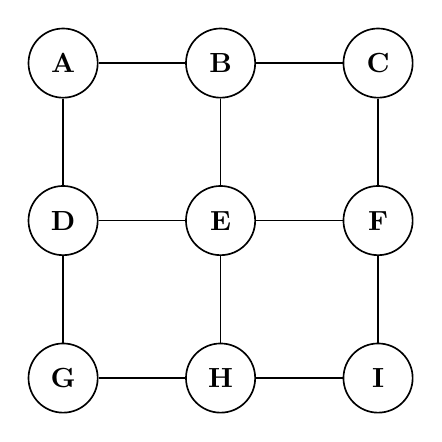
\begin{tikzpicture}[-,>=stealth',auto,node distance=2cm,semithick]
  \tikzstyle{every state}=[text=black]

  \node[state] (A) {\textbf{A}};
  \node[state] (B) [right of=A] {\textbf{B}};
  \node[state] (C) [right of=B] {\textbf{C}};
  \node[state] (D) [below of=A] {\textbf{D}};
  \node[state] (E) [right of=D] {\textbf{E}};
  \node[state] (F) [right of=E] {\textbf{F}};
  \node[state] (G) [below of=D] {\textbf{G}};
  \node[state] (H) [right of=G] {\textbf{H}};
  \node[state] (I) [right of=H] {\textbf{I}};
  
  \path (A) edge (B);
  \path (B) edge (C);
  \path (D) edge (E);
  \path (E) edge (F);
  \path (G) edge (H);
  \path (H) edge (I);
  \path (A) edge (D);
  \path (D) edge (G);
  \path (B) edge (E);
  \path (E) edge (H);
  \path (C) edge (F);
  \path (F) edge (I);
  
\end{tikzpicture}
\end{center}
\caption{The layout of Chloe Cow County}
\label{fig:county}
\end{figure}


\item After graduating from Cornell Tech, you find yourself consulting for Chloe Cow County.
In the county, there are 9 towns connected by roads in a grid as depicted in Figure~\ref{fig:county} (assume that the distance between two adjacent towns has length 1).
The county is looking to open up schools in the area, and they need your help!
Because of funding and student populations, each school must serve (exactly) two adjacent towns and each town can only send their students to a single school.
A school will be placed either in one of the two towns it serves or somewhere along the road in between the two towns.
In order to minimize travel time for its citizens, each town prefers that its school is as close to the town as possible with utility $1$ minus the distance to its school (assuming it is assigned a school to begin with). 
Note that not every town will necessarily be assigned a school.

\begin{enumerate}
\item Encode the problem as an exchange network as a way to come up with a ``stable'' way to place schools in the county.
We say that an assignment of schools as ``stable'' if no town can convince one of its neighboring towns to break away from the assignment and fund a new school with a different placement. 

Specifically, give a graph $G$ with edge values $v$, and explain how a stable outcome in $G$ corresponds to a stable assignment of schools.

\item Ignoring stability, prove that valid placement of schools must leave at least one town without a school.

\item Find a stable outcome in this graph.
You can compute the outcome either by hand or by using one of the algorithms outlined in the book.
Explain why the outcome you found is stable.

\item \textbf{Bonus:} Prove that any county with towns laid out in an $n \times m$ grid (as in the $3\times 3$ grid of Figure 1) will have a stable outcome. For which values of $n,m$ will all towns have access to a school?

\iftemplate
\begin{solution}
\begin{enumerate}
\item[9.]
\begin{enumerate}
\item[(a)]
\item[(b)]
\item[(c)]
\item[(d)] \textbf{Bonus}
\end{enumerate}
\end{enumerate}
\end{solution}
\newpage
\fi




\end{enumerate}

\item Ben Bitdiddle is running a venture capital firm that specializes in investing in early-stage video game companies. You are tasked with helping him decide which games to invest in. In particular, you are interested in \textit{social} multiplayer video games -- i.e. those video games that are fun only if groups of friends play them together.

Unfortunately the market has some pretty entrenched players: ``Chess'' and ``Among Us''. There are two new games you might want to invest in: ``Checkers'' and ``Among Stuff''. The goal is to get Chess players to switch to Checkers, and Among Us players to switch to Among Stuff. The more money Ben Bitdiddle invests in each game, the more `initial players' will play the new game. You want to know how much `initial investment' each new game might require in order to get substantial market share.

\begin{enumerate}
\item  Let's focus on Chess and Checkers. Model the `social graph' of this video game as a connected undirected graph with $n$ players, where everyone starts by playing Chess. A player will switch from Chess to Checkers if at least one of their neighbors play Checkers (i.e. maybe Checkers is a lot more fun than Chess).

Say the graph has degree $3$ (with no self-loops) and Ben Bitdiddle ``permanently sponsors'' a single initial player to play Checkers. Will everyone eventually play checkers, regardless of which player Ben sponsors? Prove your answer.


\item Among Us and Among Stuff are more social games, requiring more players. Let's say each player of Among Us has 24 friends who also play Among Us, and will switch to Among Stuff if at least 8 of their friends have already switched.

Say that Ben Bitdiddle ``permanently sponsors'' 8 initial players to play Among Stuff. Will everyone always eventually play Among Stuff? If not, describe a counterexample (for your choice of $n$). Assume as before that the graph is connected.

\end{enumerate}

\iftemplate
\begin{solution}
\begin{enumerate}
\item[10.]
\begin{enumerate}
\item[(a)]
\item[(b)]
\end{enumerate}
\end{enumerate}
\end{solution}
\newpage
\fi

\item Suppose a search engine has three ad slots that it can sell. Slot $a$ has a clickthrough rate of 6, slot $b$ has a clickthrough rate of 5, and slot $c$ has a clickthrough rate of 1. There are three advertisers who are interested in these slots. Advertiser $x$ values clicks at 4 per click, advertiser $y$ values clicks at 2 per click, and advertiser $z$ values clicks at 1 per click. 

Compute the socially optimal allocation and the VCG prices for it. Give a brief explanation for your answer.

\iftemplate
\begin{solution}
\end{solution}
\newpage
\fi

\end{enumerate}

\end{document}

